\documentclass[tikz,crop]{standalone}

\usepackage{tikz}
\usetikzlibrary{positioning}

\begin{document}
    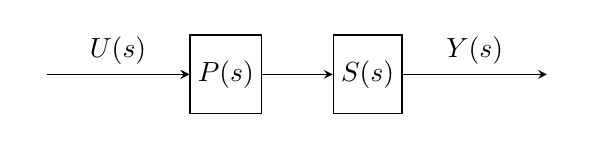
\begin{tikzpicture}[
        auto,
        >=stealth,
        on grid,
        block/.style={draw, rectangle, minimum height=10mm, minimum width=6mm, inner sep=1mm},
        sum/.style={draw, circle, inner sep=1mm},
        dot/.style={anchor=base, fill=black, circle, inner sep=0.4mm}
    ]
        \node (input) at (0,0) {};
        \node [block, right=24mm of input] (plant) {$P(s)$};
        \node [block, right=18mm of plant] (sensor) {$S(s)$};
        \node [right=24mm of sensor] (output) {};

        \draw [->] (input) -- node[above]{$U(s)$} (plant);
        \draw [->] (input) -- (plant);
        \draw [->] (plant) -- (sensor);
        \draw [->] (sensor) -- node[above, name=out]{$Y(s)$} (output);
    \end{tikzpicture}
\end{document}
